% Tipo de documento (presentación)
\documentclass[usenames,dvipsnames]{beamer}

% Cargar el tema
\usetheme{metropolis}

% Configuración de LaTeX
\usepackage[spanish]{babel}
\usepackage[utf8]{inputenc}

\usepackage{listings}

\usepackage{color}
\definecolor{grisclarito}{gray}{0.95}

\lstdefinestyle{customc}{
  %belowcaptionskip=1\baselineskip,
  breaklines=true,
  frame=single,
  %xleftmargin=\parindent,
  language=C,
  showstringspaces=false,
  basicstyle=\ttfamily\tiny,
  keywordstyle=\bfseries\color{green!40!black},
  commentstyle=\itshape\color{purple!40!black},
  identifierstyle=\color{blue},
  stringstyle=\color{orange},
  backgroundcolor=\color{grisclarito}
}
\lstdefinestyle{custompython}{
  %belowcaptionskip=1\baselineskip,
  breaklines=true,
  frame=single,
  %xleftmargin=\parindent,
  language=Python,
  showstringspaces=false,
  %basicstyle=\ttfamily,
  keywordstyle=\bfseries\color{green!40!black},
  commentstyle=\itshape\color{purple!40!black},
  identifierstyle=\color{blue},
  stringstyle=\color{orange},
  backgroundcolor=\color{grisclarito}
}

\lstdefinestyle{customhtml}{
  %belowcaptionskip=1\baselineskip,
  breaklines=true,
  frame=single,
  %xleftmargin=\parindent,
  language=HTML,
  showstringspaces=false,
  %basicstyle=\ttfamily,
  keywordstyle=\bfseries\color{green!40!black},
  commentstyle=\itshape\color{purple!40!black},
  identifierstyle=\color{blue},
  stringstyle=\color{orange},
  backgroundcolor=\color{grisclarito}
}



\usepackage{graphicx,wrapfig,lipsum}
\graphicspath{{./imagenes/}}

% Configuración básica del tema
\metroset{
  % tema oscuro ('dark') o claro ('light'). No tiene efecto al usar la
  % paleta de colores más adelante
  background=light,
  % 'none' para eliminar la diapositiva inicial de cada sección
  sectionpage=progressbar,
  % 'progressbar' o 'simple' para añadir una diapositiva inicial a cada subsección
  subsectionpage=none,
  % contador de página: 'none', 'counter' o 'fraction'
  numbering=none,
  % barra de progreso: 'none', 'head', 'frametitle' o 'foot'
  progressbar=frametitle,
  % fondo de los bloques estilo teorema: 'transparent' o 'fill'
  block=fill,
}
\usepackage{amsmath,amsthm,verbatim,amssymb,amsfonts,amscd, graphicx}
\usetikzlibrary{babel}
\usepackage{pgfplots}
\usepackage{booktabs}
\usepackage{float}
\usepackage{enumitem}
\usepackage{forest}
\usepackage{hyperref}
\usepackage{gnuplottex}
\graphicspath{{./imagenes/}}
\usepackage{csvsimple}
\usepackage{multicol}

% Paleta de colores
\definecolor{accent}{RGB}{151, 186, 88}
\colorlet{darkaccent}{accent!70!black}
\definecolor{foreground}{RGB}{0, 0, 0}
\definecolor{background}{RGB}{255, 255, 255}

% Insertar los colores en el tema
\setbeamercolor{normal text}{fg=foreground, bg=background}
\setbeamercolor{alerted text}{fg=darkaccent, bg=background}
\setbeamercolor{example text}{fg=foreground, bg=background}
\setbeamercolor{frametitle}{fg=background, bg=accent}

\setbeamercolor{headtitle}{fg=background!70!accent,bg=accent!90!foreground}
\setbeamercolor{headnav}{fg=background,bg=accent!90!foreground}
\setbeamercolor{section in head/foot}{fg=background,bg=accent}

%
\defbeamertemplate*{headline}{miniframes theme no subsection}{
  % Caja para mostrar título y autor encima de cada diapositiva
  % Nosotros no 
  %% \begin{beamercolorbox}[ht=2.5ex,dp=1.125ex,
  %%     leftskip=.3cm,rightskip=.3cm plus1fil]{headtitle}
  %%   {\usebeamerfont{title in head/foot}\insertshorttitle}
  %%   \hfill
  %%   \leavevmode{\usebeamerfont{author in head/foot}\insertshortauthor}
  %% \end{beamercolorbox}
  %% \begin{beamercolorbox}[colsep=1.5pt]{upper separation line head}
  %% \end{beamercolorbox}

  % Caja para mostrar navegación encima de cada diapositiva
  \begin{beamercolorbox}{headnav}
    \vskip2pt\insertnavigation{\paperwidth}\vskip2pt
  \end{beamercolorbox}
  \begin{beamercolorbox}[colsep=1.5pt]{lower separation line head}
  \end{beamercolorbox}
}

%eye-candy; sintasix más bonita
\newcommand{\seccion}[1]{\input{./sections/#1}}
\newcommand{\foo}{\hspace{-2.3pt}$\bullet$ \hspace{5pt}}

%Meta
\title{Comunicación bidireccional en arquitecturas cliente/servidor}
\subtitle{El protocolo \textbf{WebSocket}}
\date{\today}
\institute{Universidad de Granada}
\author{Juan Francisco Díaz Moreno \\ Javier Sáez de la Coba}



\usepackage{graphicx}
\begin{document}
\maketitle
\begin{frame}{Contenidos.}
  \setbeamertemplate{section in toc}[sections numbered]
  \tableofcontents [hideallsubsections]
\end{frame}

\section{Introducción. }
%\subsection{intro} %Ponemos la subseccion para que nos aparezcan los circulos de progesion
\begin{frame}{Arquitectura Cliente-Servidor. }

En arquitecturas cliente-servidor siempre es el cliente el que pide cosas al servidor.
\begin{figure}[H]

	\begin{center}
	\includegraphics[scale=0.3]{imagenes/client-serer.png}
	\end{center}
	
\end{figure}

\end{frame}

\begin{frame}{Arquitectura Cliente-Servidor. }

¿Que ocurriría si es el servidor el que le quiere mandar información al cliente sin que este se lo pida?

\end{frame}

\begin{frame}{Solución. }

\begin{center}\huge{WebSockets}\end{center}

\end{frame}

\begin{frame}{WebSockets. }

WebSockets es un protocolo de comunicaciones cliente-servidor full-dúplex incluido en el estándar HTML5

\end{frame}

\section{Evolución histórica}
%\subsection{hola}

\begin{frame}{Inicios de la Web}

	\begin{center}
	\includegraphics[scale=0.45]{imagenes/first_web.jpg}
	\end{center}
	
\end{frame}

\begin{frame}{Dinamismo}

	\begin{center}
	\huge{JavaScript}
	\end{center}
	
\end{frame}

\begin{frame}{Webs como aplicaciones}

	\begin{center}
	\huge{IFrames como módulos de las apps}
	\end{center}
	
\end{frame}


\begin{frame}{Servidor -> Cliente}

	\begin{center}
	\huge{HTTP Polling}
	\end{center}
	
\end{frame}

\begin{frame}{Servidor -> Cliente}

	\begin{center}
	\huge{LiveConnect}
	\end{center}
	
\end{frame}


\begin{frame}{Servidor -> Cliente}

	\begin{center}
	\huge{Forever Frame}
	\end{center}
	
\end{frame}

\begin{frame}{Servidor -> Cliente}

	\begin{center}
	\huge{Long Polling}
	\end{center}
	
\end{frame}

\begin{frame}{Servidor -> Cliente}

	\begin{center}
	\huge{SSE}
	\end{center}
	
\end{frame}

\begin{frame}{Tecnologías actuales}

	\begin{center}
	\includegraphics[scale=0.29]{imagenes/sse-xhr-ws.png}
	\end{center}
	
\end{frame}




\section{Protocolo WebSockets} %%%%%%%%%%%%%%%%%%%%%%%
%\subsection{hola}
\begin{frame}{WebSockets. }

WebSocket es una tecnología que proporciona un canal de comunicación bidireccional sobre un único socket TCP.

Está diseñada para ser implementada en navegadores y servidores web.

Con esta API, puede enviar mensajes a un servidor y recibir respuestas controladas por eventos sin tener que consultar al servidor para una respuesta.

\end{frame}

\begin{frame}

Los WebSockets necesitan ser implementados tanto del lado del cliente como del servidor.

En el lado del cliente, está ya implementado en Mozilla Firefox 8, Google Chrome 4, Safari 5; así como en la versión móvil de Safari en el iOS 4.2 y en el Internet Explorer 10.

\centering
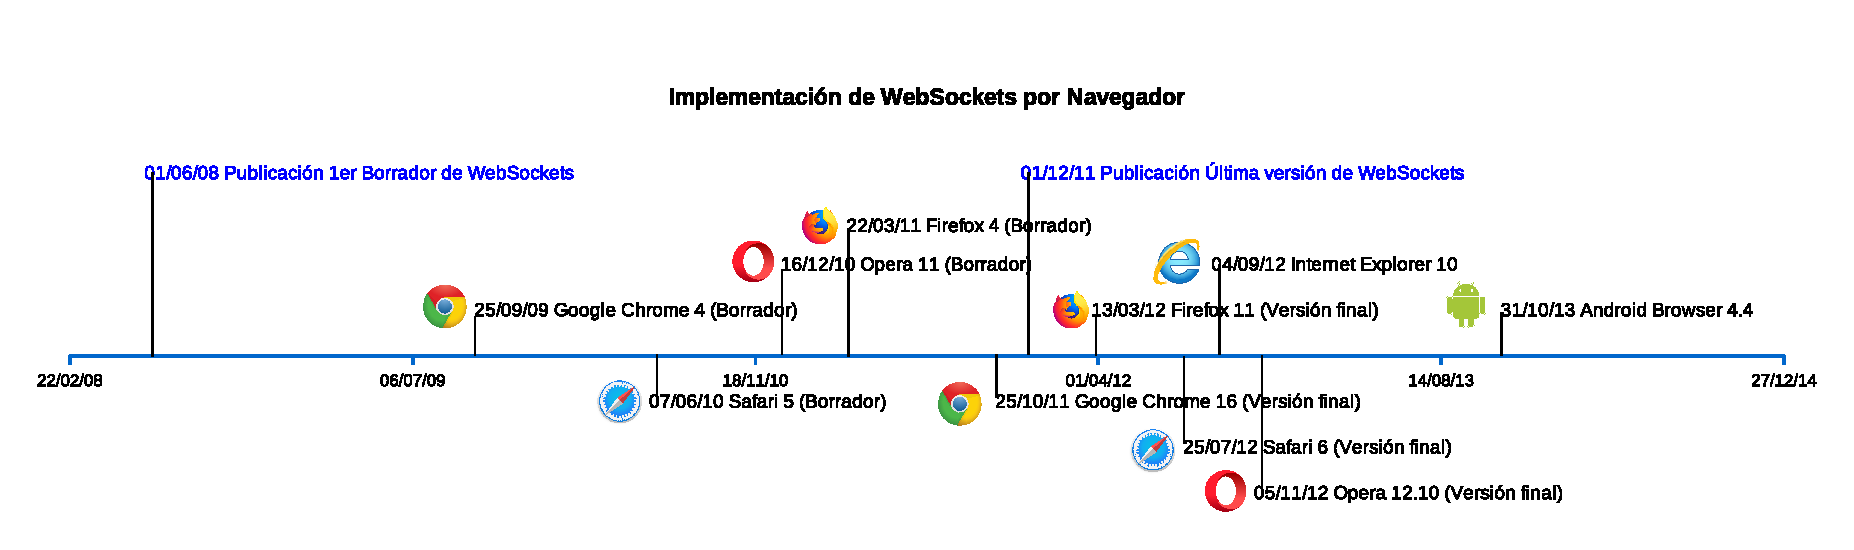
\includegraphics[scale=0.35]{imagenes/timeline.pdf}

\end{frame}



\begin{frame}{Ejemplos de WebSockets.}


	\begin{center}
	\includegraphics[scale=0.29]{imagenes/whatsapp.png}
	\end{center}

\end{frame}

\begin{frame}{Ejemplos de WebSockets.}


	\begin{center}
	\includegraphics[scale=0.29]{imagenes/facebook.png}
	\end{center}

\end{frame}

\begin{frame}{Ejemplos de WebSockets.}


	\begin{center}
	\includegraphics[scale=0.29]{imagenes/netflix.png}
	\end{center}

\end{frame}

\begin{frame}{Ejemplos de WebSockets.}


	\begin{center}
	\includegraphics[scale=0.29]{imagenes/bet365.png}
	\end{center}

\end{frame}

\begin{frame}{Ejemplos de WebSockets.}


	\begin{center}
	\includegraphics[scale=0.29]{imagenes/github.png}
	\end{center}

\end{frame}

\begin{frame}{Ejemplos de WebSockets.}


	\begin{center}
	\includegraphics[scale=0.29]{imagenes/sharelatex.png}
	\end{center}

\end{frame}

\section{Utilidad de los WebSockets}

\begin{frame}
WebSockets tiene una gran cantidad de ventajas entre las que destacan:
\begin{itemize}
\item Comunicación full-duplex entre cliente y servidor.
\item Mejora la eficiencia de la comunicación cliente-servidor, estableciendo una única conexión.
\item Estandariza las comunicaciones evitando soluciones propietarias.
\item API bien documentada y fácil de implementar e integrar en nuestras aplicaciones.
\item Permite crear aplicaciones modernas con requerimientos de comunicación en tiempo real.
\end{itemize}
\end{frame}

\begin{frame}
	WebSockets se implementa de lado de cliente en JavaScript pero necesita soporte de lado de servidor. Una gran cantidad de lenguajes de programación permiten el uso de WebSockets, permitiendo crear servidores de aplicaciones en el lenguaje que queramos. Un ejemplo de estos lenguajes que soportan WebSockets son: C, JavaScript, Python, Ruby, Haskell, Java, PHP, Objetive-C, Swift...
\end{frame}

\section{Descripción de una conversación WebSockets. }
%\subsection{intro} %Ponemos la subseccion para que nos aparezcan los circulos de progesion
\begin{frame}{Conversación WebSocket }

\begin{figure}[H]
\centering
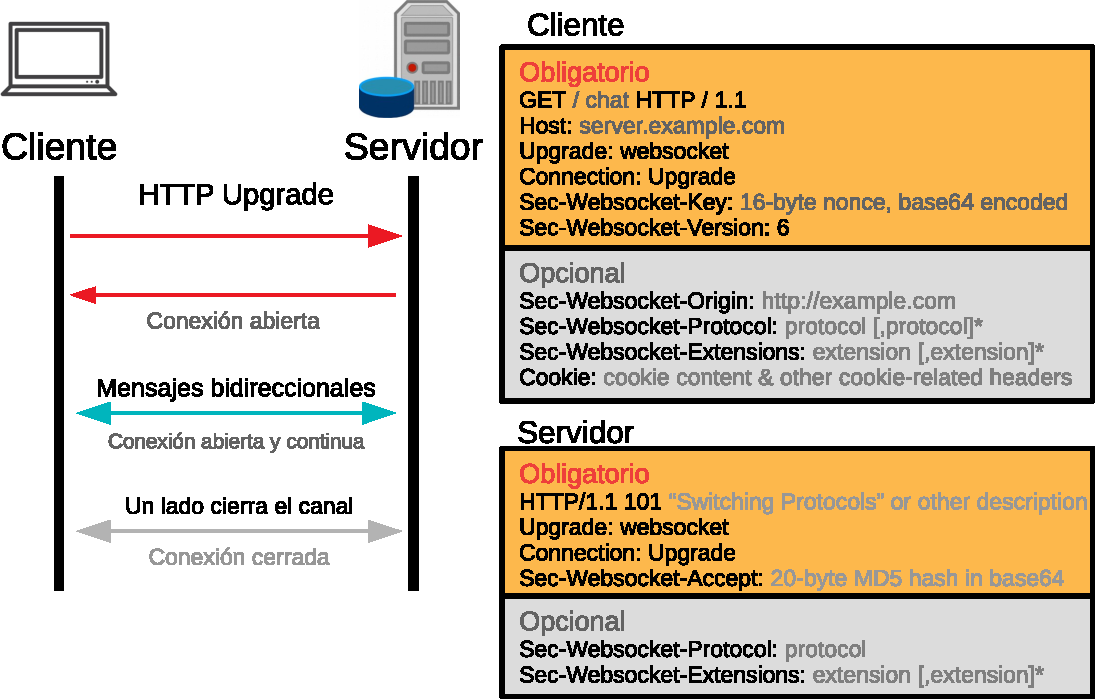
\includegraphics[scale=0.5]{imagenes/diagrama.pdf}
\end{figure}
\end{frame}

\section{Implementación de una app usando WebSockets. }
%\subsection{intro} %Ponemos la subseccion para que nos aparezcan los circulos de progesion
\begin{frame}{Conversación WebSocket }

\begin{figure}[H]
\centering
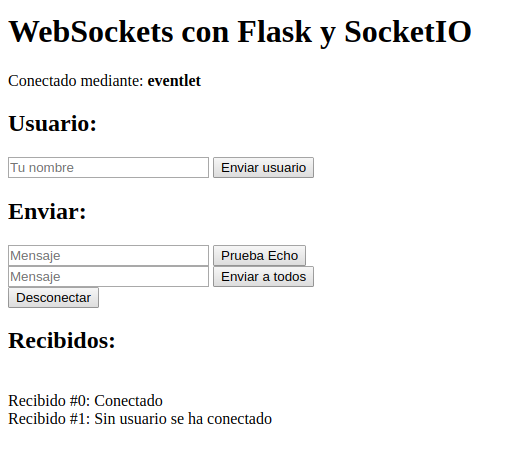
\includegraphics[scale=0.5]{imagenes/app.png}
\end{figure}
\end{frame}

\begin{frame}{Código}

	\begin{center}
	\huge{Código fuente de la app}
	\end{center}
	
\end{frame}

\begin{frame}{Live Demo}

	\begin{center}
	\huge{\url{jscoba.com:5000}}
	\end{center}
	
\end{frame}

\begin{frame}{Conversación WebSocket }

\begin{figure}[H]
\centering
\includegraphics[scale=0.5]{imagenes/wireshark.png}
\end{figure}
\end{frame}


\begin{frame}[standout]
  ¿PREGUNTAS?
\end{frame}

\begin{frame}[standout]
  FIN
\end{frame}

\end{document}
